\documentclass{article}

% if you need to pass options to natbib, use, e.g.:
%     \PassOptionsToPackage{numbers, compress}{natbib}
% before loading neurips_2018

% ready for submission
% \usepackage{neurips_2018}

% to compile a preprint version, e.g., for submission to arXiv, add add the
% [preprint] option:
%     \usepackage[preprint]{neurips_2018}

% to compile a camera-ready version, add the [final] option, e.g.:
\usepackage[final]{projects}

% to avoid loading the natbib package, add option nonatbib:
%\usepackage[nonatbib]{neurips_2018}

\usepackage[utf8]{inputenc} % allow utf-8 input
\usepackage[T1]{fontenc}    % use 8-bit T1 fonts
\usepackage{hyperref}       % hyperlinks
\usepackage{url}            % simple URL typesetting
\usepackage{booktabs}       % professional-quality tables
\usepackage{amsfonts}       % blackboard math symbols
\usepackage{nicefrac}       % compact symbols for 1/2, etc.
\usepackage{microtype}      % microtypography
\usepackage{amsmath}
\usepackage{graphicx}
\usepackage{dsfont}
\usepackage{subcaption}
\usepackage{MnSymbol}%
\usepackage{wasysym}%

\usepackage{mathtools}

\usepackage[ruled]{algorithm2e}

\newtheorem{theorem}{Theorem}
\newtheorem{definition}{definition}
\newtheorem{lemma}{Lemma}
\newtheorem{proof}{Proof}[section]




\title{Policy Iteration through evolutionary function approximation}

\author{%
  Yunian Pan \\
  Department of Electrical Engineering \\ 
  \texttt{yp1170@nyu.edu} 
}

\begin{document}

\maketitle

\begin{abstract}
  This report presents the substances of the paper "Evolutionary Function Approximation for Reinforcement Learning", along with some
  simulations using the related algorithm. In the context that temporal difference methods are theoretically grounded and empirically effective methods for addressing reinforcement learning problems,
 we have been moving towards a era of deep learning that in most real-world reinforcement learning tasks, 
TD methods require a function approximator to represent the value function. However, using function approximators
 requires manually making crucial representational decisions. The related papers investigates evolutionary function approximation, 
 a novel approach to automatically selecting function approximator representations that enable efficient individual learning. 
 The method, which naturally arises from genetic algorithm schemes, evolves individuals that are better able to learn. 
 
 Some implemented instantiations of evolutionary function approximation which combines NEAT, a neuroevolutionary optimization technique,
  with Q-learning, a popular TD method was presented in paper $^{[1]}$, The resulting NEAT+Q algorithm automatically discovers effective
  representations for neural network function approximators. The original paper also presents on-line evolutionary computation, which improves
   the on-line performance of evolutionary computation by borrowing selection mechanisms used in TD methods to choose individual actions
    and using them in evolutionary computation to select policies for evaluation. 

  Also some online searching scheme has been proposed in this paper based on epsilon greedy method or Boltzmann distribution, which improves 
  the on-line performance of evolutionary computation by borrowing selection mechanisms used in TD methods to choose individual actions 
  and using them in evolutionary computation to select policies for evaluation. Two empirical experiments were evaluated and discussed
  in this paper, it also presents additional tests that offer insight into what factors can make neural network function approximation difficult in practice.


\end{abstract}

\section{Introduction}
Reinforcement learning problems are the subset of machine learning tasks in which the agent never sees examples of correct behavior. Instead, it receives only positive and negative rewards for the actions it tries.
 Since many practical, real world problems (such as robot control, game playing, and system optimization) fall in this category, developing effective reinforcement learning algorithms is critical to the 
 progress of artificial intelligence.

 The most common approach to reinforcement learning relies on the concept of value functions, which indicate, for a particular policy, the long-term value of a given state or state-action pair. Temporal difference methods (TD($\lambda$)) (Sutton, 1988),
which combine principles of dynamic programming with statistical sampling, use the immediate rewards received by the agent to incrementally improve both the agent’s policy and the estimated 
 value function for that policy. Hence, TD methods enable an agent to learn during its “lifetime” i.e. from its individual experience interacting with the environment.

When the problem scale is not large, the value function can be represented as a table of state-action pairs, but for large scale systems or for problems that has infinite dimension of 
state space or action space, it remains problematic to only use a "table", instead the function approximator which represents the mapping from state-action pairs to values via a more concise,
parameterized function and uses supervised learning methods to set its parameters, plays an important role where we can omit the step of enumering over
the state-action space.  Many different methods of function approximation have been used successfully, including CMACs, radial basis functions, and neural networks.

However, using function approximators requires making crucial representational decisions (e.g. the number of hidden units and ini- tial weights of a neural network. 
Poor design choices can result in estimates that diverge from the optimal value function and agents that perform poorly. Even for reinforcement learning algorithms 
with guaranteed convergence, achieving high performance in practice requires finding an appropriate representation for the function approximator. 

As Lagoudakis and Parr observe,$^{[1]]}$ “The crucial factor for a successful ap- proximate algorithm is the choice of the parametric approximation architecture(s) and the choice of the projection (parameter adjustment) method.” (Lagoudakis and Parr, 2003, p. 1111) Nonetheless, representational choices are typically made manually, based only on the designer’s intuition.

Therefore, in order to automate the search for effective representations by employing sophisticated optimization techniques, we focus on using evolutionary methods 
because of their demonstrated ability to discover effective representations, so that our proposition can cover the 2 things: 1) an evolutionary algorithm capable of optimizing representations from a class of functions; 2) a TD method that uses elements of that class for function approximation. 

Neural network is a good choice as hey have great experimental value, Nonlinear function approximators are often the most challenging to use, hence, success for evolutionary function approximation with neural networks is good reason to hope for success with linear methods too;
and they have great potential in that they can represent value functions that the linear method cannot(given the same basis functions). Therefore NeuroEvolution of Augmenting Topologies(NEAT)$^{[2]]}$ has been chosen as the main 
framework. The resulting algorithm, called NEAT+Q, uses NEAT to evolve topologies and initial weights of neural networks that are better able to learn, via backpropagation, to represent the value estimates provided by Q-learning.

Section 2 will present the background including Q-learning and deep Q-learning, genetic algorithms and NEAT framework and NEAT algorithm for reinforcement learning and some basic related experiments;
Section 3 will present the new emerging method that incorporates the previous algorithm together, along with the experiments and discussion.
Section 4 will have some discussion over the results obtained from the experiments.

\section{Background}
This section mainly contains two parts, one is for the development of Q-learning, Deep Q learning, and some variance of them; The another will discuss the 
machinery and framework and using NEAT to do reinforcement learning, specifically, we will start from the general framework of genetic algorithm and with a little bit discussion
on how it works, then introduce a gene encoding scheme that NEAT relies on.
\subsection{Q-learning}

As a model-free algorithm, Q-learning trains the agent what action to take under what circumstances, is a well-established, canonical method that has also enjoyed empirical success,
In the tabular case, the algorithm is defined by the following update rule, applied each time the agent transitions from state s to state $s^{\prime}$:
\begin{equation}
   Q(s,a ) = (1 - \alpha) Q(s, a) + \alpha( r + \gamma  \min_{a^{\prime}}Q(s^{\prime} ,a^{\prime}) ) \label{q}
\end{equation}
where $\alpha \in [0, 1]$ is a learning rate parameter, $\gamma \in [0, 1]$ is a discount factor, and $r$ is the immediate reward the agent receives upon taking action $a$.

This equation was initially derived from Bellman equation regarding Markov Decision Process, recall the original operator of value function:
\begin{equation}
  (TJ)(i) : = \min_{u \in U(i)} \sum_{j=1}^{n} p_{ij}(u)[g(i,u,j)+ \alpha J(j)]
\end{equation} 
define: $Q(s,a) = \sum_{j=1}^{n} p_{ij}(u)[g(i,u,j)+ \alpha J(j)]$, we can omit the probability transition, and through Robins-Monro algorithm
we solve the Q-learning problem and end up with the update rule $\ref{q}$.

 
 \subsection{Q-Learning with NN}

 Particularly when combined with neural network function approximators, 
 algorithm $\ref{1}$ describes the Q-learning algorithm using a neural network to approximate the value function. The inputs to the network describe the agent’s current state; the outputs,
  one for each action, represent the agent’s current estimate of the value of the associated state-action pairs. 
  The initial weights of the network are drawn from a Gaussian distribution with mean $0$ and standard deviation $\sigma$ (line 5). 
 The EVAL-NET function returns the activation on the network’s outputs after the given inputs are fed to the network and propagated forward. Since the network uses a sigmoid activation function,
  these values will all be in $[0,1]$ and hence are rescaled according to a parameter $c$. The parameter $\lambda$ the sample roll-out cost decay, which is for the convenience of
  doing $TD(\lambda)$ extension, which we usually set to 0 or 1, respectively representing the value iteration method and the policy evaluation method.

   \begin{algorithm}[H] 
     \caption{Q-Learning}
     \label{1}
     \KwIn{$S:$ set of all states; $A:$ set of all actions; $\sigma:$ standard deviation of initial weights; 
     $c:$ output scale; $\alpha:$ learning rate; $\gamma:$ discount factor; $\lambda:$ eligibility decay rate; 
     $\epsilon_{td}:$ exploration rate; $e:$ total number of episodes;}
     \textbf{Initialize:} $N \leftarrow$ INIT-NET$(S,A,\sigma)$ \;    
     \For{ $i \leftarrow 1 $ to $e$ }{$s, s^{\prime} \leftarrow $ null, INIT-STATE($S$)\;
     \While{Terminal-state?(s)}{
       $Q[] \leftarrow c \times $EVAL-NET$(N,s^{\prime})$\;
       \textbf{With-prob}($\epsilon_{td}$) $a^{\prime} \leftarrow$ RANDOM$(A)$\;
       \textbf{else:} $a^{\prime} \leftarrow \arg\max Q[j]$\;
       \eIf{$s \neq null $}
       {BACKPROP$(N,s,a,(r + \gamma \max_{j} Q[j])/ c, \alpha, \gamma, \lambda)$ \;}
       {$s, a \leftarrow s^{\prime}, a^{\prime}$\;
       $r, s^{\prime} \leftarrow$ TAKE-ACTION$(a^{\prime})$}
     }
     }
     \end{algorithm}

\subsection{NEAT}
\subsubsection{genetic algorithm}

Genetic algorithm(GA) is a metaheuristic inspired by the process of natural selection that belongs to the larger class of evolutionary algorithms(EA).
Genetic algorithms are commonly used to generate high-quality solutions to optimization and search problems by relying on bio-inspired operators such as mutation, crossover and selection.$^{[3]}$
\begin{figure}[htbp]
  \centering
  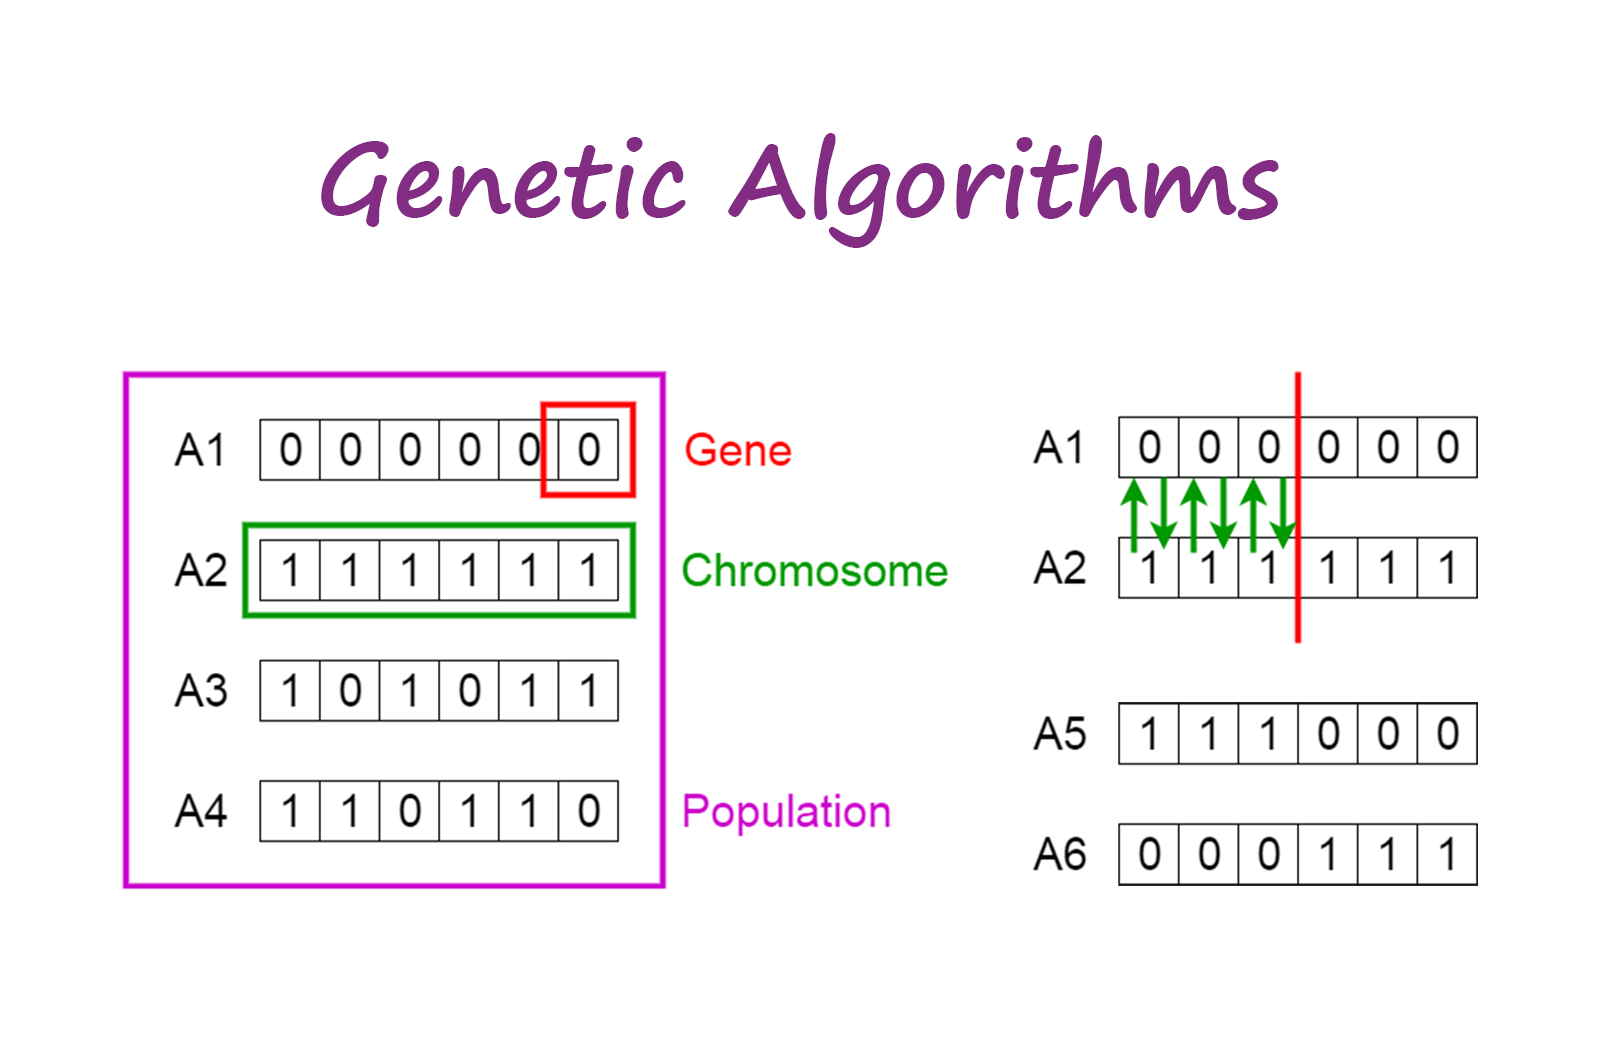
\includegraphics[width = .7\textwidth]{illu.png}
  \caption{from Google Image}
  \label{illu}
\end{figure}
Figure $\ref{illu}$ describes a simple case of doing one iteration gene evolution, the binary codes in the left side represent the population of solutions to the objective problem, while the right side
illustrates the process of doing crossover, the mutation step left is just randomly change the 1's into 0's. The convergence is guaranteed under the condition that we choose the best species at 
every generation.

A standard evolution framework can be summarized as:
\begin{itemize}
  \item[(1)] Initialize population
  \item[(2)] Evolve from $1, \ldots, n_{generation}$:
  \begin{itemize} 
  \item[a)] Select from population according to \underline{fitness}
  \item[b)] Generate offspring through \underline{crossover} and \underline{mutation}
  \item[c)] Replace population with offspring. 
  \end{itemize}
\end{itemize}
The flow chart $\ref{flow}$ describes the scheme:
\begin{figure}[htbp]
  \centering
  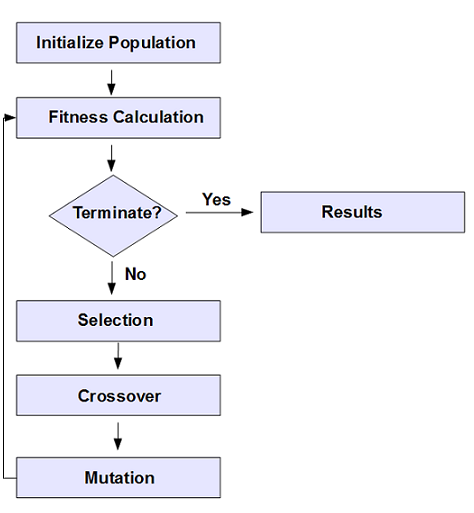
\includegraphics[width = .6\textwidth]{genetic}
  \caption{from Google Image}
  \label{flow}
\end{figure}
Inspired by the framework, one might think about apply it to finding the best structure of a neural network, i.e. we initialize a population
of neural networks, then proceed the nature selection based on the fitness of the networks and try to breed the next generation with the winners,
iteratively increasing the fitness of each generation until the resulting population satisfies the performance criterion. 


\subsubsection{Another TWEANN encoding}

In order to develop the neural evolution algorithm, we need a standard method to encode the neural networks as genotypes so that we can
do crossover and mutation operation based on the genotypes provided. There are many evolutionary systems of neural networks while Topology and Weight Evolving Artificial Neural Networks(TWEANN)
encoding is the best approach to address the question of how to encode networks using an efficient genetic representation. Absorbing the properties of
many TWEANN systems, NEAT encodes the neural networks in following ways:

\begin{figure}[htbp]
  \centering
  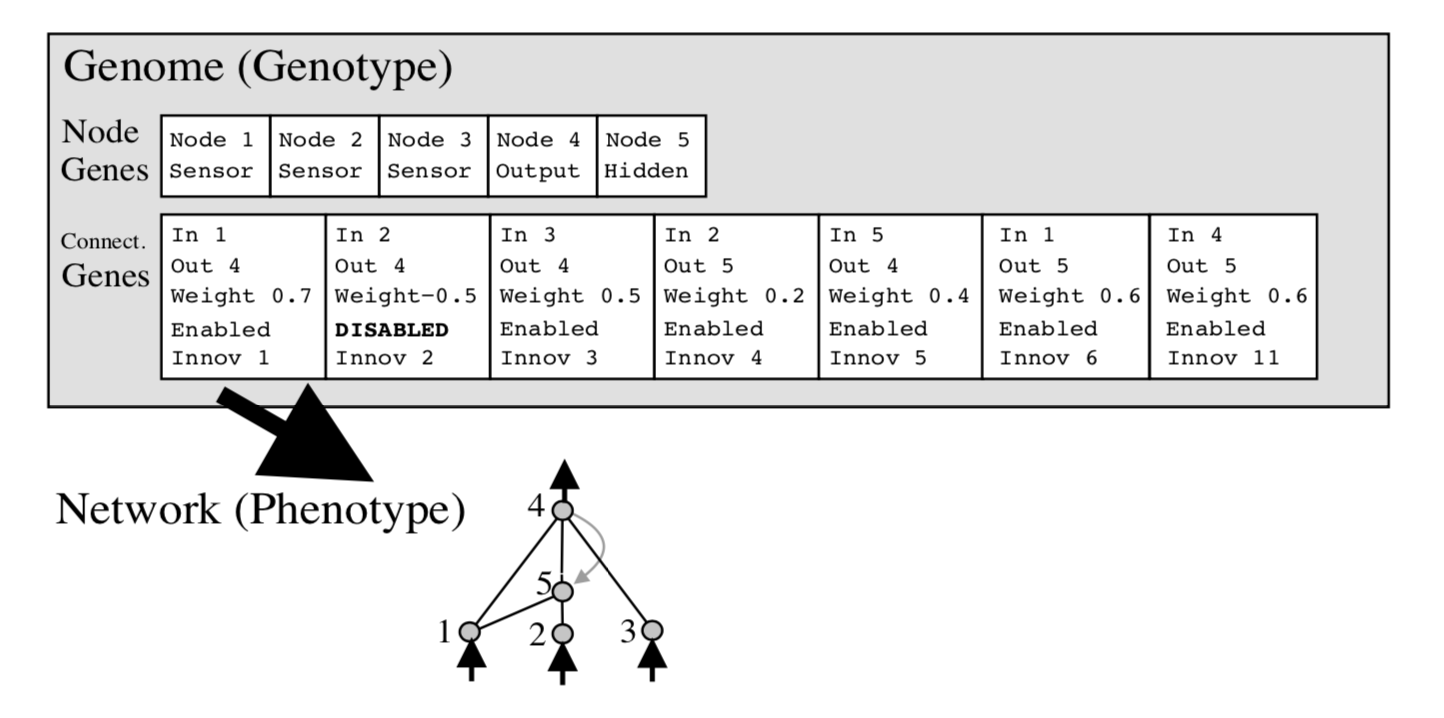
\includegraphics[width = .8\textwidth]{genome}
  \caption{genotype and phenotype from $^{[2]}$}
  \label{genotype}
\end{figure}

Genomes in NEAT are linear representations of network connectivity. 

The figure $\ref{genotype}$ illustrates a genotype to phenotype mapping example. A genotype is depicted that produces the shown phenotype. There are 3 input nodes, one hidden, and one output node, and seven connection definitions,
 one of which is recurrent. The second gene is disabled, so the connection that it specifies (between nodes 2 and 4) is not expressed in the phenotype.

 \begin{figure}[htbp]
  \centering
  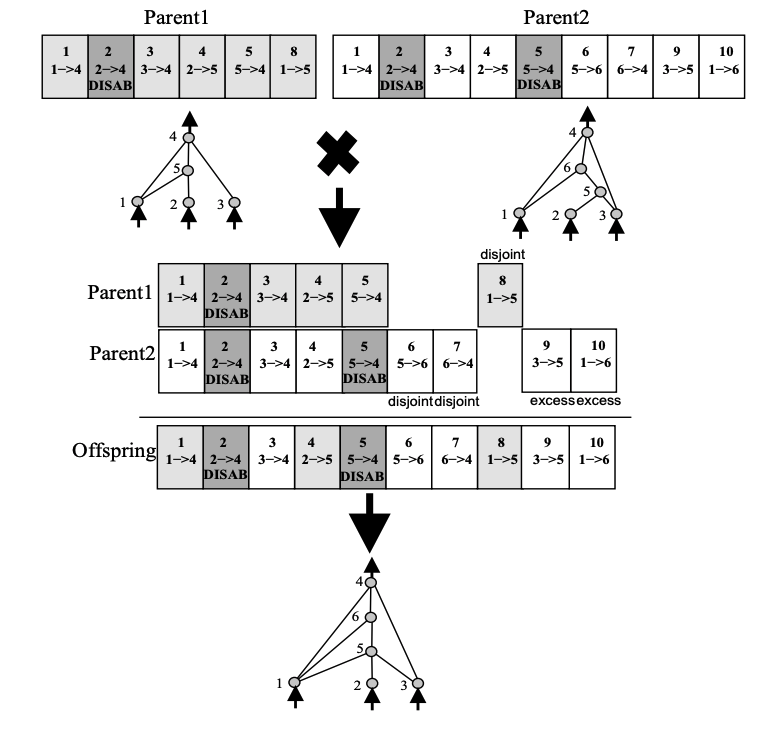
\includegraphics[width = .8\textwidth]{crossover}
  \caption{crossover from $^{[2]}$}
  \label{crossover}
\end{figure}

The figure $\ref{crossover}$ illustrates Matching up genomes for different network topologies using innovation numbers. 
 Parent 1 and Parent 2's innovation numbers (shown at the top of each gene) tell us which genes match up with which. Even without any topological analysis,
 a new structure that combines the overlapping parts of the two parents as well as their different parts can be created. Matching genes are inherited randomly, whereas disjoint genes (those that do not match in the middle)
  and excess genes (those that do not match in the end) are inherited from the more fit parent. In this case, equal fitnesses are assumed, so the disjoint and excess genes are also inherited randomly. 
  The disabled genes may become enabled again in future generations: there’s a preset chance that an inherited gene is disabled if it is disabled in either parent.

  Figure $\ref{mutation}$ illustrates the two types of structural mutation in NEAT. Both types, adding/deleting a connection and adding/deleting a node, are illustrated with the connection genes of a network shown above their phenotypes. 
  The top number in each genome is the innovation number of that gene. The innovation numbers are historical markers that identify the original historical ancestor of each gene.
   New genes are assigned new increasingly higher numbers.
\begin{figure}[htbp]
    \centering
    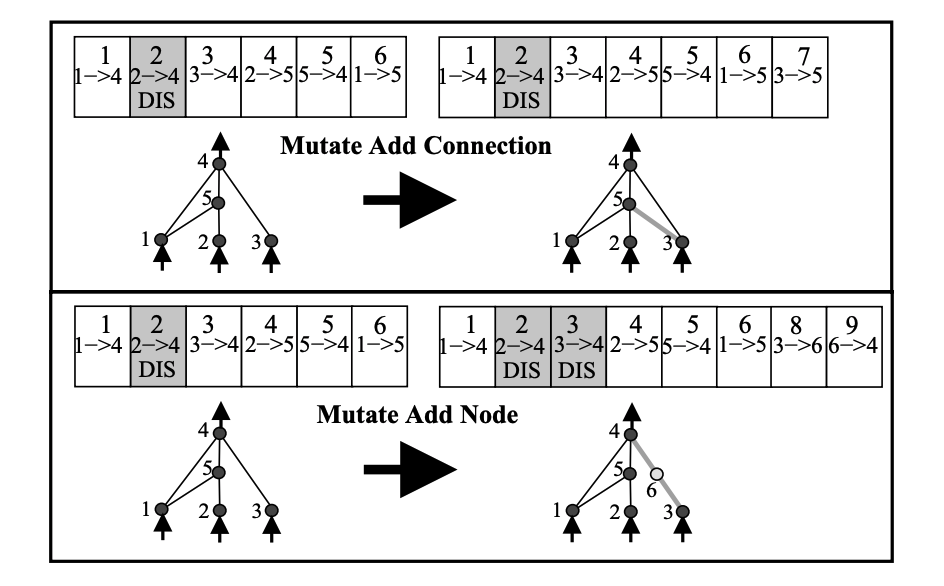
\includegraphics[width = .8\textwidth]{mutation}
    \caption{mutation from $^{[2]}$}
    \label{mutation}
  \end{figure}
  To be noted, NEAT begins with a uniform population of simple networks with no hidden nodes and inputs connected directly to outputs.


\subsubsection{NEAT algorithm}
Without the aid of TD methods, namely Q-learning, NEAT can tacle reinforcement learning in that NEAT does not attempt to learn a value function but tries to find good policies directly by training action selectors,
which map states to the action the agent should take in that state, as the same as we do in policy evaluation reinforcement learning, which uses the global optimizing 
techniques that directly search the space of potential policies.

Algorithm $\ref{neat}$ contains a high-level description of the NEAT algorithm applied to an episodic reinforcement learning problem. It differs from 
the original algorithm in that for every step of choosing network for policy evaluation, the network is not chosen from directly the fixed order of
population vector, but randomly selected. This change does not significantly alter NEAT’s behavior but facilitates to excel online by balancing exploration and exploitation within and across generations.

\begin{algorithm}[H]
  \label{neat}
  \caption{NEAT($S, A, p , m_n, m_l, g, e$)}
  \KwIn{$S$:set of all states, $A$:set of all actions, $p$:population size , $m_n$: rate of adding node, $m_l$: rate of adding link, $g$: generations, $e$: episodes;}
  \textbf{Initialize:} $P[] \leftarrow$ Init-Populations$(S,A,p)$ \;    
  \For{ $i \leftarrow 1 $ to $g$ }{\For{$j \leftarrow 1 $ to $e$}{
  $N, s, s^{\prime} \leftarrow $ Random($P$), null, INIT-STATE($S$)\;
  \While{Terminal-state?(s)}{
    $Q[] \leftarrow  $EVAL-NET$(N,s^{\prime})$\;
    $a^{\prime} \leftarrow \arg\max Q[j]$;  $\quad$
    $s, a \leftarrow s^{\prime}, a^{\prime}$;  $\quad$
    $r, s^{\prime} \leftarrow$ TAKE-ACTION$(a^{\prime})$\;
    $N.fitness \leftarrow N.fitness + r$
    }
    $N.episodes \leftarrow N.episodes + 1$
    }
  $P^{\prime} \leftarrow$ new array of size p\;
  \For{$j \leftarrow 1 $ to $p$}{
    $P^{\prime}[] \leftarrow$  Breed-Net$(P[])$\;
    \textbf{with-probability} $m_n$: ADD-Node-Mutation($P^{\prime}[j]$)\;
    \textbf{with-probability} $m_l$: ADD-link-Mutation($P^{\prime}[j]$)
  }
  $P[] \leftarrow P^{\prime}[]$
  }
  \end{algorithm}

\subsubsection{speciation}
In most cases, adding new structure to a network initially reduces its fitness.
However, NEAT speciates the population, so that individuals compete primarily within their own niches rather than with the population at large.
Hence, topological innovations are protected and have time to optimize their structure before competing with other niches in the population.

Historical markings make it possible for the system to divide the population into species based on topological similarity. 
The distance $\delta$ between two network encodings is a simple linear combination of the number of excess (E) and disjoint (D) genes, as well as the average weight differences of matching genes (W):
\begin{equation}
 \delta = \frac{c_1 E}{N} + \frac{c_2 D}{N}  + c_3 \bar{W}
\end{equation}
where the coefficients $c_1, c_2$ and $c_3$ adjust the importance of the three factors, and the factor $N$, the number of genes in the larger genome, normalizes for genome size.

\subsection{NEAT+Q algorithm}

Since all that is required to make NEAT optimize value functions instead of action selectors is a reinterpretation of its output values, the output of
the neural network is alreay identical to what the Q value function represents. Therefore, if the weights of the networks NEAT evolves are updated during their fitness evaluations using Q-learning and backpropagation, 
they will effectively evolve value functions instead of action selectors. 

\begin{algorithm}[H]
  
  {\tiny\caption{NEAT+Q($S, A, p , m_n, m_l, g, e$)}}
  \KwIn{$S$, $A$, $p$, $m_n$, $m_l$, $g$, $e$, $\alpha$, $\lambda$, $\gamma$, $\epsilon$}
  \textbf{Initialize:} $P[] \leftarrow$ Init-Populations$(S,A,p)$ \;    
  \For{ $i \leftarrow 1 $ to $g$ }{\For{$j \leftarrow 1 $ to $e$}{
  $N, s, s^{\prime} \leftarrow $ Random($P$), null, INIT-STATE($S$)\;
  \While{Terminal-state?(s)}{
    $Q[] \leftarrow  $EVAL-NET$(N,s^{\prime})$\;
    \textbf{With-prob}($\epsilon_{td}$) $a^{\prime} \leftarrow RANDOM(A)$\;
    \textbf{else:} $a^{\prime} \leftarrow \arg\max Q[j]$\;
    \If{$s \neq null $}
    {$BACKPROP(N,s,a,(r + \gamma \max_{j} Q[j])/ c, \alpha, \gamma, \lambda)$}
    $s, a \leftarrow s^{\prime}, a^{\prime}$\;
    $r, s^{\prime} \leftarrow$ TAKE-ACTION$(a^{\prime})$\;
    $N.fitness \leftarrow N.fitness + r$
    }
    $N.episodes \leftarrow N.episodes + 1$
    }
    $P^{\prime} \leftarrow$ new array of size p\;
    \For{$j \leftarrow 1 $ to $p$}{
      $P^{\prime}[] \leftarrow$  Breed-Net$(P[])$\;
      \textbf{with-probability} $m_n$: ADD-Node-Mutation($P^{\prime}[j]$)\;
      \textbf{with-probability} $m_l$: ADD-link-Mutation($P^{\prime}[j]$)
    }

  }
  \end{algorithm}

  To be noted there are two kinds of implementations of NEAT+Q, one is Lamarkian in which the weights are inherited by the next generation, one is Darwinian in which
  the weights are not. Results will show that there's no advantage in each of them.



\subsection{$\epsilon$ greedy selection and Boltzmann selection}

The algorithm has variant versions in that during the online choosing step we can use either $\epsilon$ greedy selection or Boltzmann selection, as we know that 
in the TD method the step forward process is done by balancing the exploration and exploitation tradeoff using the two selection methods, in particular the 
probability distribution is constructed using the Q value function:

  $$\Pr(\cdot| s) = \frac{e^{Q(s,\cdot)/\tau}}{\sum_{a\in A} e^{Q(s,a)/\tau}}$$

It's remarkable that we can borrow the Boltzmann selection and the $\epsilon$ greedy selection in the exploration and exploitation tradeoff acrossing the generations,
only by replacing the Q function with fitness function:

  $$\Pr(\cdot) = \frac{e^{S(\cdot)/\tau}}{\sum_{q\in P} e^{S(q)/\tau}}$$

  where $S(q)$ is the average fitness of the policy $q$ represented by the neural network, $\tau$ is the Boltzmann temperature, as $\tau$ goes to 0,
  the selection becomes greedy, otherwise completely random.

Thus regarding the online step variantion, take the Boltzmann selection for example, should be:
\begin{algorithm}[H]
  {\tiny\caption{Boltzman Selection($P, \tau$)}}
  \KwIn{$P:$ population, $\tau$: softmax temperature}
    \eIf{$\exists N \in P \ |\ N.episodes = 0 $}
    {return $N$}
    {$total \leftarrow \sum_{N \in P} e^{N.average / \tau}$\;
    \For{$N\in P$}{
      with-prob ($\frac{e^{N.average/\tau}}{total}$) return $N$
      else $total \leftarrow total - e^{N.average /\tau}$
    }
    }
  \end{algorithm}

\section{Experiments results}

\subsection{Mountain car task and server job scheduling task}
In the mountain car task depicted in Figure $\ref{mountaincar}$, an agent strives to drive a car to the top of a steep mountain. 
The car cannot simply accelerate forward because its engine is not powerful enough to overcome gravity. Instead, the agent must learn to drive backwards up the hill behind it, 
thus building up sufficient inertia to ascend to the goal before running out of speed.
\begin{figure}[htbp]
  \centering
  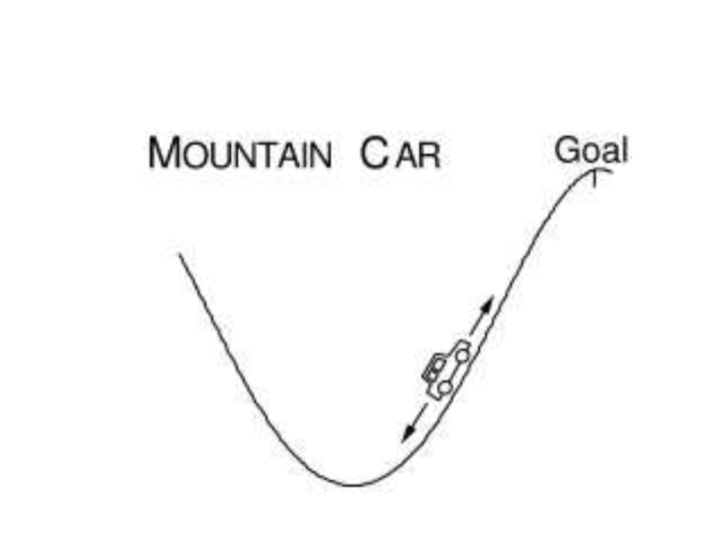
\includegraphics[width = .5\textwidth]{Mountaincar.png}
  \caption{figure from $^{[1]}$}
  \label{mountaincar}
\end{figure}

In the server job scheduling task, which is used to assess whether the methods can scale to a much more complex problem, a server, such as a website’s application server or database, 
must determine in what order to process the jobs currently waiting in its queue. Its goal is to maximize the aggregate utility of all the jobs it processes. 
A utility function for each job type maps the job’s completion time to the utility derived by the user.
 The problem of server job scheduling becomes challenging when these utility functions are nonlinear and/or the server must process multiple types of jobs.

\subsection{Comparisons}
Several comparisons regarding the comparisons between different version of algorithms are listed in this section:
\subsubsection{Manually and evolutionary}
In both domains of tasks, evolutionary function approximation significantly improves performance over manually designed networks, as shown in $\ref{neatq}$
\begin{figure}[htbp]
  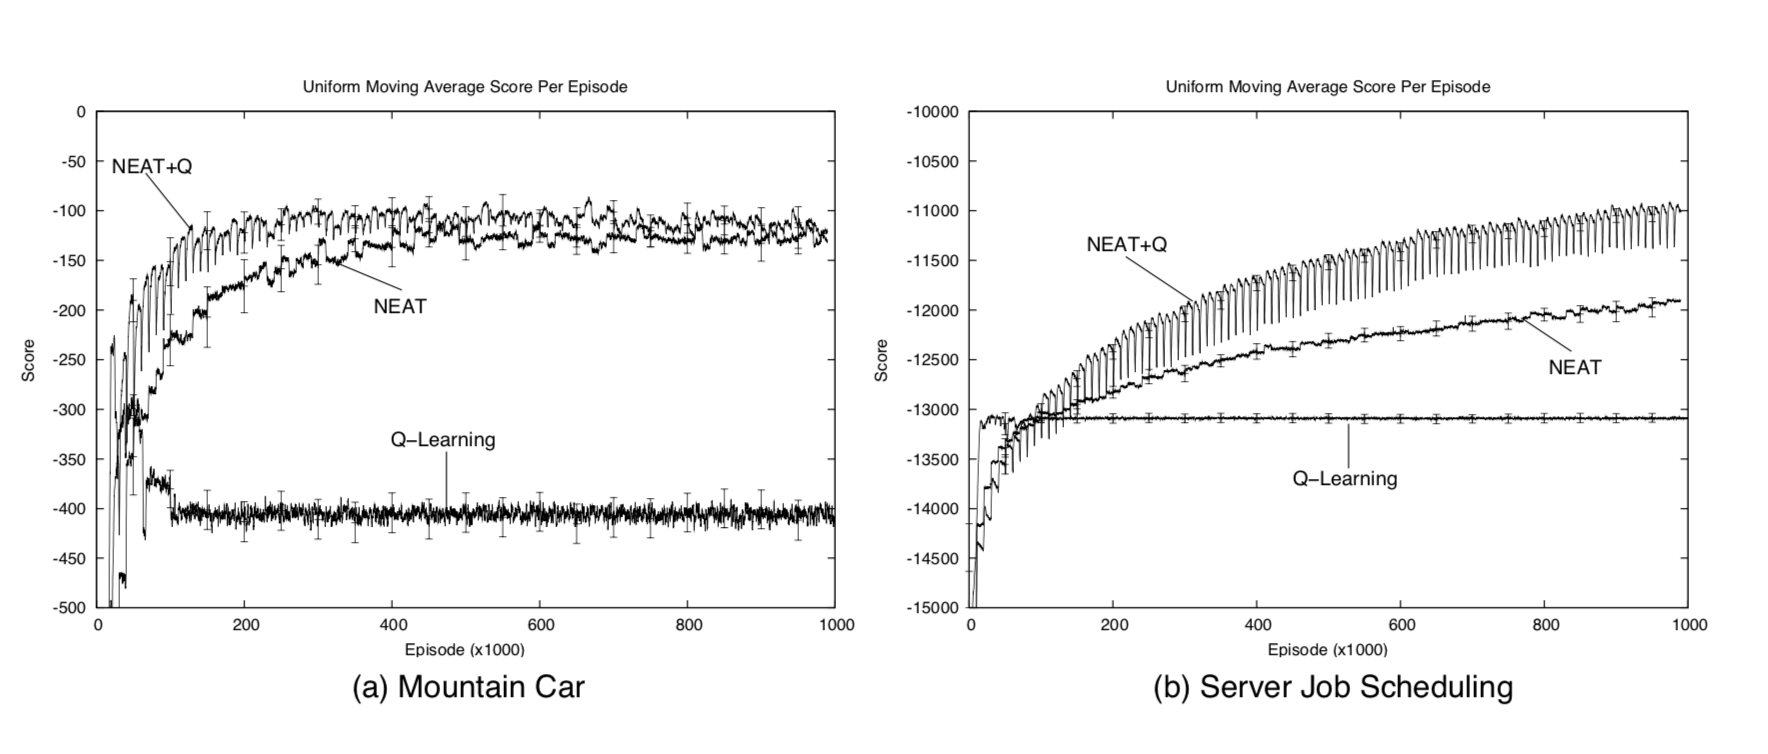
\includegraphics[width = \textwidth]{3result}
  \caption{performance of the three algorithms}
  \label{neatq}
 \end{figure}


\subsubsection{softmax and off-line}
As for on-line v.s. off-line, the softmax scheme significantly outperformsthe off-line algorithm as shown in $\ref{softmax}$, original paper also 
explored the comparison between $\epsilon$ greedy and softmax, surprisingly they perform just closely to each other.
\begin{figure}[htbp]
  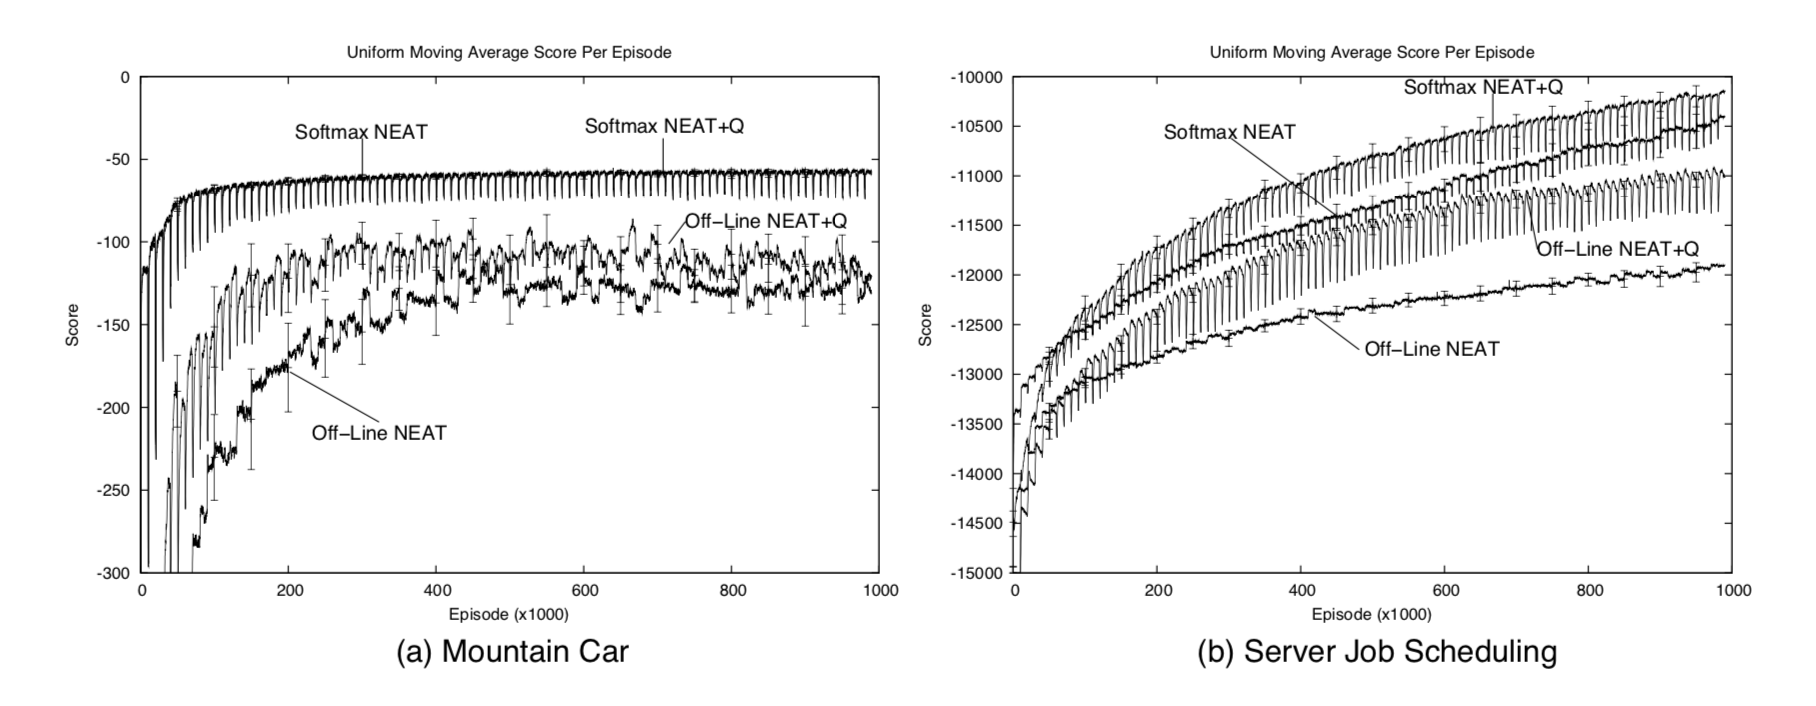
\includegraphics[width = \textwidth]{explorationneat}
  \caption{performance of Softmax and off-line NEAT+Q}
  \label{softmax}
 \end{figure}


\subsubsection{Lamarkian and Darwinian}
Since evolutionary function approximation can be implemented in either a Darwinian or Lamarckian fashion, the two approaches empirically in both the mountain car and server job scheduling domains
were compared. However, it is not clear that this approach is superior even though it more closely matches biological systems, as shown in $\ref{darwinian}$
\begin{figure}[htbp]
  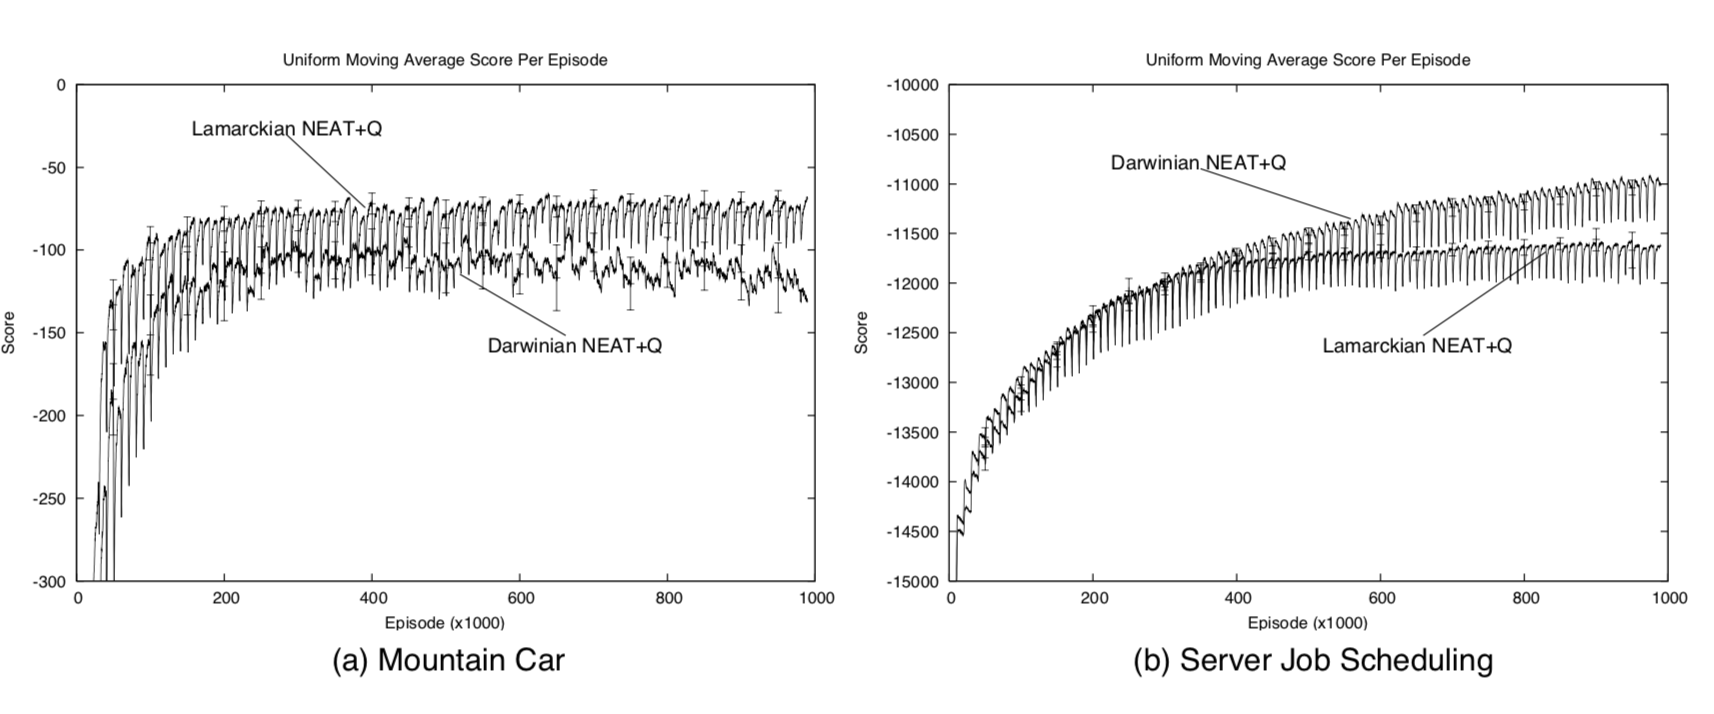
\includegraphics[width = \textwidth]{darwinian}
  \caption{performance of Darwinian and Lamarckian NEAT+Q}
  \label{darwinian}
 \end{figure}

\subsubsection{annealing and not annealing}
Two scenarios, one where the learning rate is annealed to zero after 100 episodes, just as in training, the other where it is not annealed at all were compared in 
original paper, it's remarkable that under the condition without annealing the learning rate, the online scheme actually performs worse, while with annealing the
learning rate will eliminate this phenomenon.
\begin{figure}[htbp]
  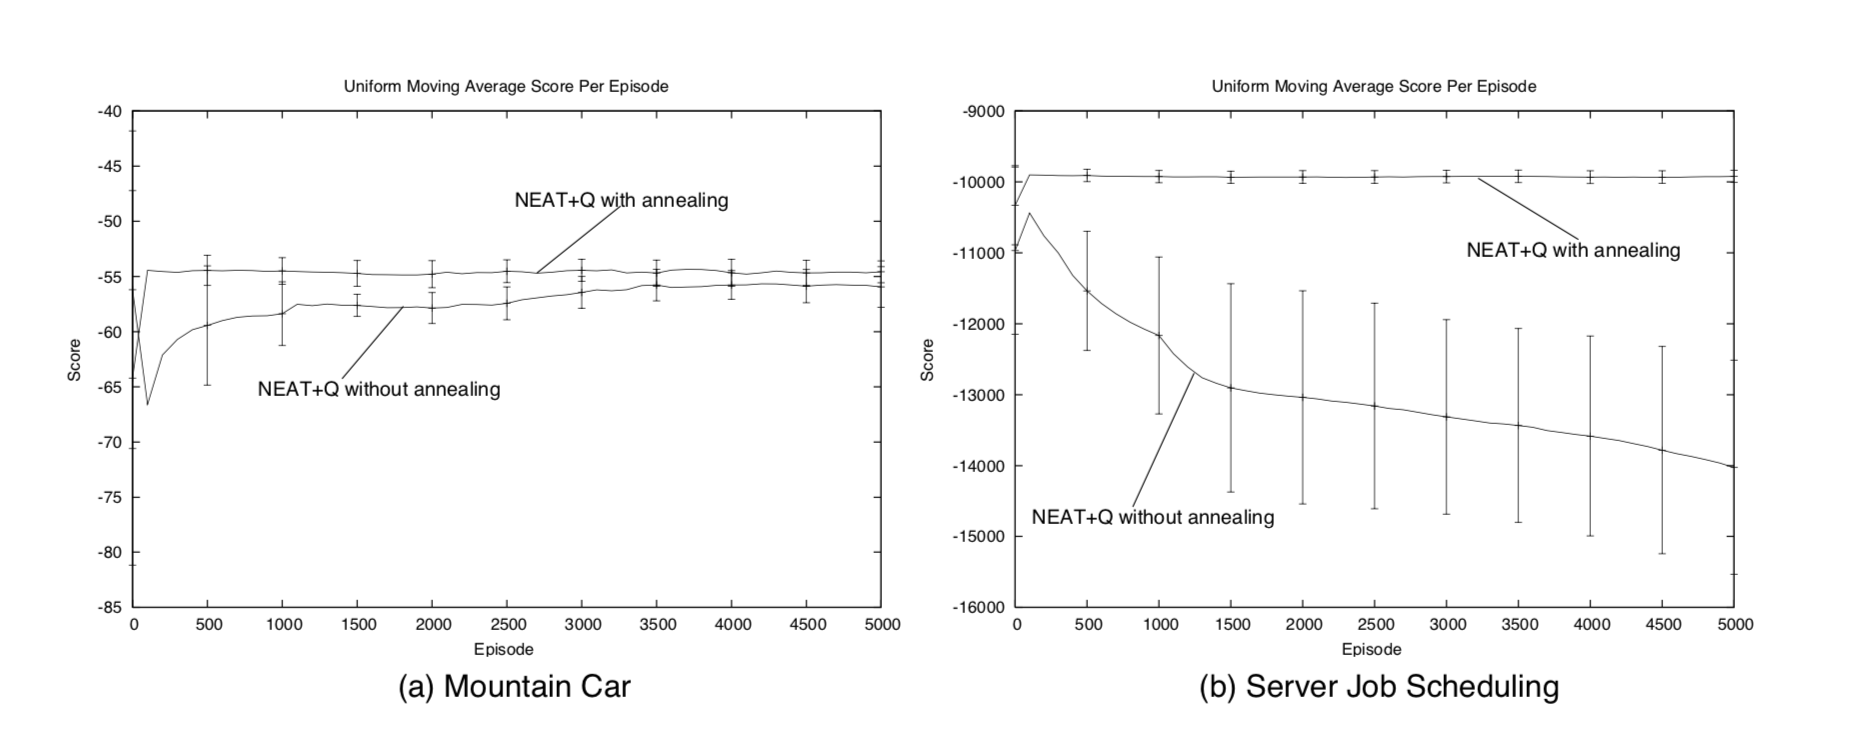
\includegraphics[width = \textwidth]{anneal}
  \caption{}
 \end{figure}


 
\section{Simulations and comparison}
There are some of the results demonstrated with an emphasis on NEAT algorithm.

\subsection{Cartpole}

In order to illustrate how simple the structure that NEAT automatically searched is, the first environment we tested is the cartpole, also known as the inverted pendulum, 
 the observation space is consist of 4 variables, corresponding to 4 dimensional inputs, and the action space consisting of 2 elements.
 we simply set the initial neural network to be with 4 inputs and 2 outputs, with no hidden layers. 
 
 As $\ref{learn1}$ shows, we are able 
 to find the best individuals from the population within 2 generations, partially because neural network has been achieved great success 
 and simplicity of the environment model. The final winner's structure is as shown in $\ref{evo1}$, is surprisingly simple as red lines indicate that
 the connectivity is enabled.

 Table $\ref{table1}$ shows some basic configuration that was used for NEAT.

 \begin{table}[htbp]
  \caption{parameter setting}
  \label{table1}
  \centering
  \begin{tabular}{llllll}
    \toprule
    %\multicolumn{5}{c}{}                   \\
    \cmidrule(r){1-6}
   population size & mutation rate & Node add/delete    & Connection add/delete    & activation & elitism  \\
    \midrule
   100 & $0.1$ &  $0.9/0.2$  & $0.9/0.1$ & relu &  2    \\
        \bottomrule
  \end{tabular}
\end{table}

\begin{figure}[htbp]
  \centering
  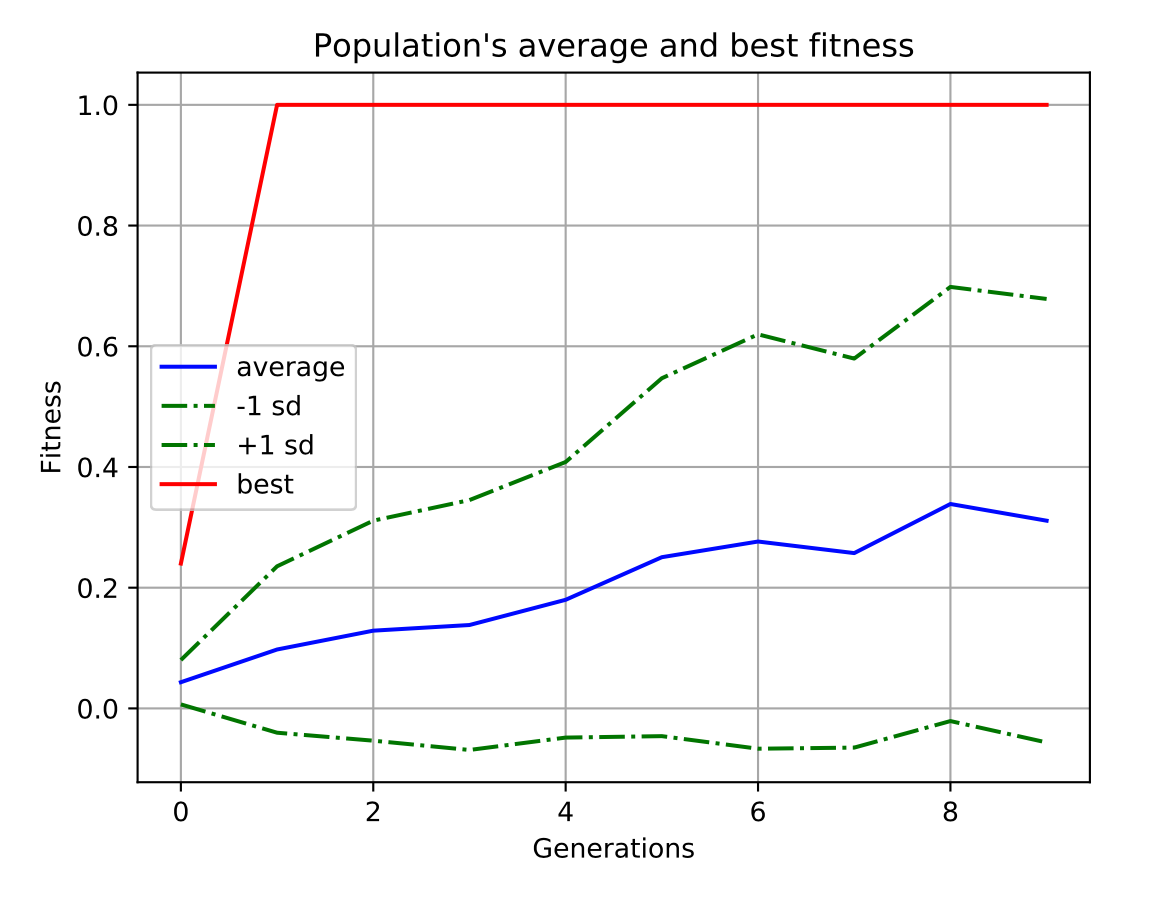
\includegraphics[width = .6\textwidth]{fitness_cartpole}
  \caption{Learning curve of cart pole}
  \label{learn1}
 \end{figure}

 \begin{figure}[htbp]
  \centering
  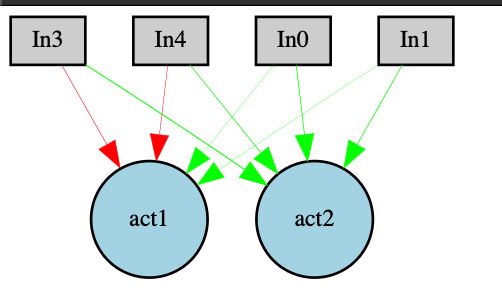
\includegraphics[width = .5\textwidth]{network_cartpole}
  \caption{Final conectivity of Cart pole}
  \label{evo1}
 \end{figure}

 As a comparison, if we change the hidden layer into 1, the learning curve becomes $\ref{learn3}$, which means the manually determined structure
 could slow down the automate search.

 \begin{figure}[htbp]
  \centering
  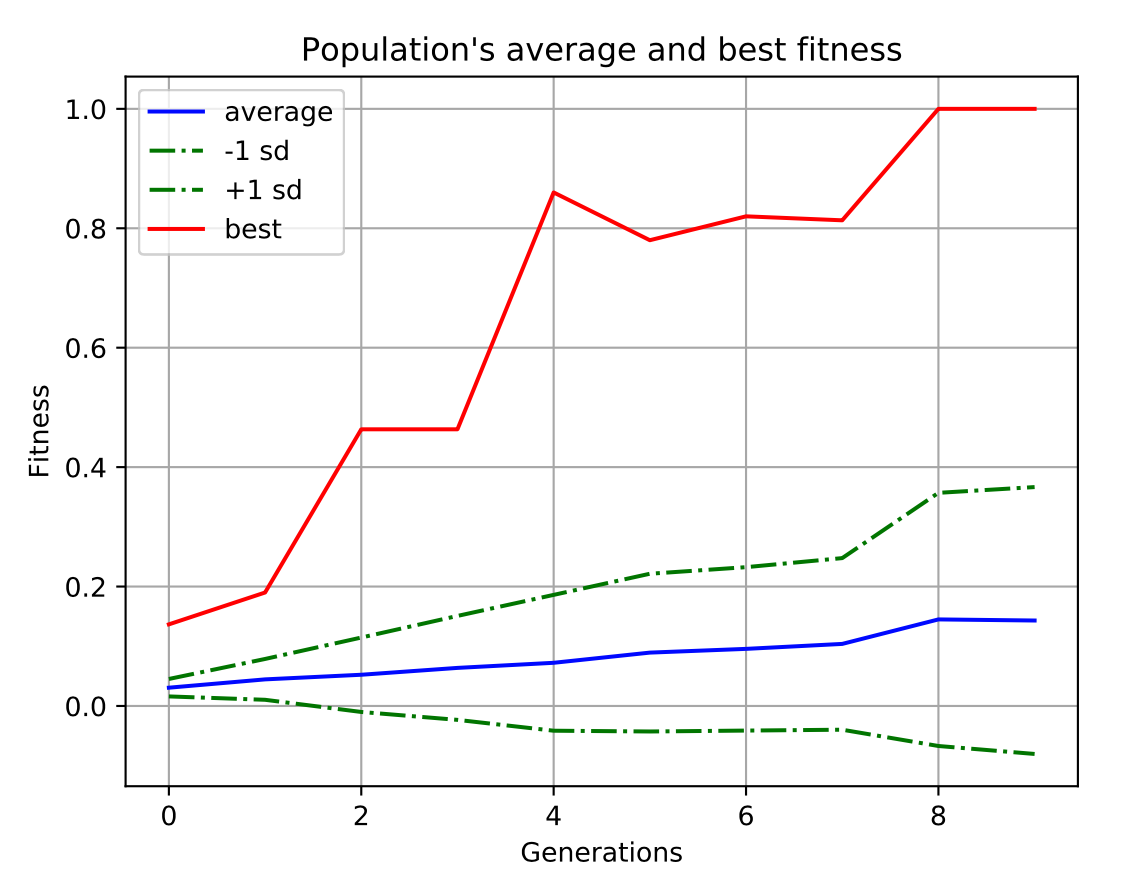
\includegraphics[width = .5\textwidth]{learn3}
  \caption{learning curve of cart pole with 1 hidden layer initialized}
  \label{learn3}
 \end{figure}

\subsection{Atari game: Pac-man}
An environment with larger complexity called Pac Man has also been tested using the NEAT algorithm, in this environment,
the observation space is 128 dimensional, the action space is 9 dimensional, therefore we set the initial structure to have
128 inputs with 9 dimensional sigmoid outputs, and 8 hidden layers, table $\ref{table2}$ shows the basic configuration of
neat algorithm:

\begin{table}[htbp]
  \caption{parameter setting}
  \label{table2}
  \centering
  \begin{tabular}{llllll}
    \toprule
    %\multicolumn{5}{c}{}                   \\
    \cmidrule(r){1-6}
    population size & mutation rate & Node add/delete    & Connection add/delete    & activation & elitism  \\
    \midrule
    150&$0.1$ &  $0.9/0.2$  & $0.25/0.1$ & relu &  2    \\
        \bottomrule
  \end{tabular}
\end{table}

After 1000 generations of training, each generation contains variant episodes within which my action in the environment will be finished,
learning curve is just shown in Figure $\ref{learn2}$.

\begin{figure}[htbp]
  \centering
  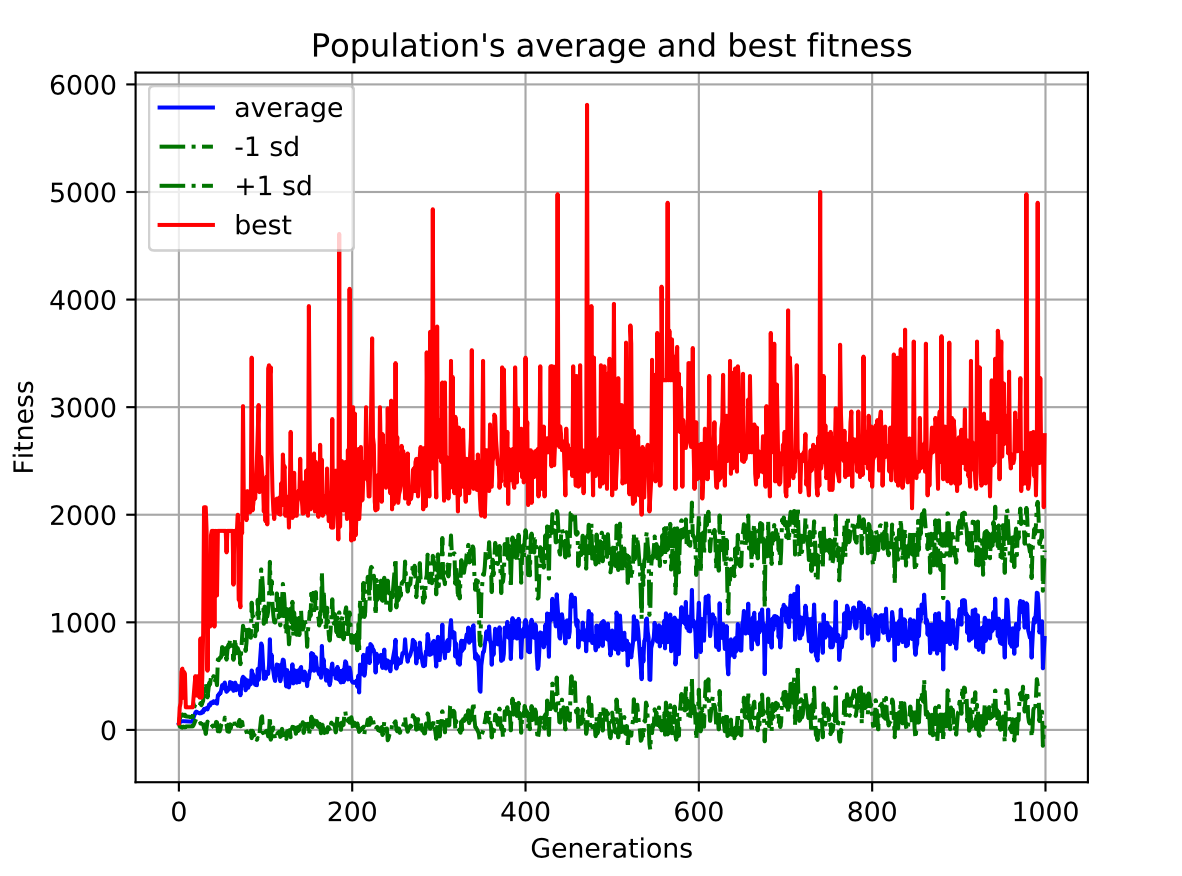
\includegraphics[width = .7\textwidth]{fitness_atari}
  \caption{Learning curve of Pac-man}
  \label{learn2}
 \end{figure}

 \begin{figure}[htbp]
  \centering
  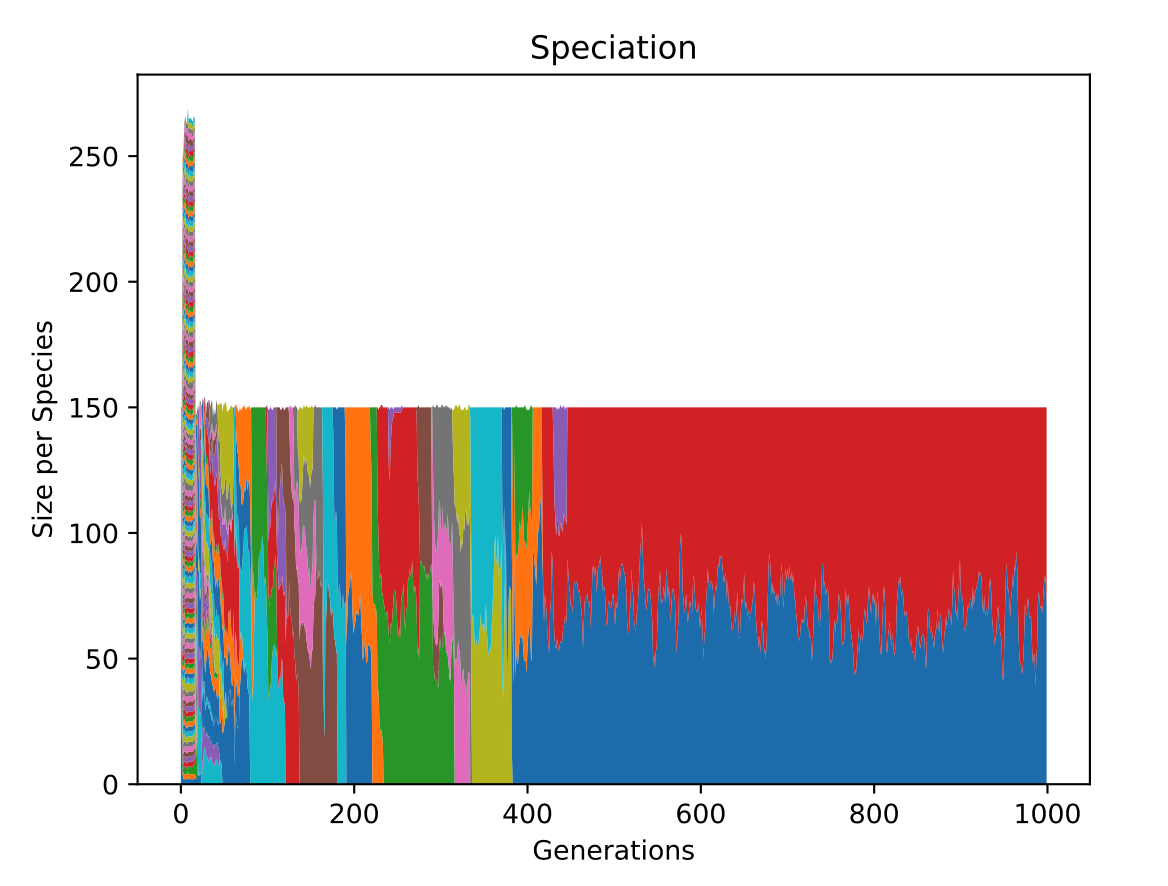
\includegraphics[width = .7\textwidth]{speciation_atari}
  \caption{Evolution diagram of Pac-man}
  \label{evo2}
 \end{figure}
 Limited by the scale of graph, the connectivity is not shown here, instead the species' evolution
 is shown, from which we can observe that there are initially very dense species, as the generation goes,
 the genetic distance between species will be closer and the genomes keep competing with each other within their
 genetic niches, finally the 2 elite species which survived the best in the environment will be chosen left.

 

\subsection{compare to Q-learning}

In both cases the NEAT algorithm significantly outperform DQN. As we manually determine the network structure, take cart pole for e.g.,
the network defined contain 3 hidden layers with 8, 16, 8 nodes respectively, the speed of training was remarkablely slow compare to NEAT(requires above 5000 episodes while NEAT only required 10 generations);
As for in the Atari game case, both algorithms are unable to training a action selector that tacle the game, while NEAT perform better: end up with
210 reward and DQN ended up with 70 reward. The reason for this phenomenon might be because of the on-stationary environment, as in the Atari game,
the ghost can be conceived as some randomness that the states doesn't consider, yet it's rather difficult to enumerate the states that absorbing the randomness.


\section{Conclusion}

Having evidences listed before, we can summarize that :
\begin{itemize}
  \item NEAT outperform Q-learning in episodes, Generally, NEAT+Q can perform better as shown in the mountain car and server job scheduling domain; 
  \item NEAT explore the function representation automatically, similar to exploring a better policy, the episodes of ficticious play is equivalent to what we do during policy evaluation,
  only different in that the policy is hidden beneath the represented function of neural network, and we have multiple choice when it comes to policy update.
  \item It's safe to anticipate that some other Methods(DDQN and Duel QN) can be combined with NEAT, but in order to in corporate with those tools we have to add properties to the existing NEAT system
  so that it can perform backpropagation.
  \item  although the training process might work in some deterministic systems, it is still challenging to tacle non-stationary environment as the action selector only take 
  the current states into consideration.
\end{itemize}


\section*{References}

\small

[1] Whiteson, Shimon, and Peter Stone. "Evolutionary function approximation for reinforcement learning." Journal of Machine Learning Research 7.May (2006): 877-917.

[2] Stanley, Kenneth O., and Risto Miikkulainen. "Efficient reinforcement learning through evolving neural network topologies." Proceedings of the 4th Annual Conference on Genetic and Evolutionary Computation. Morgan Kaufmann Publishers Inc., 2002.

[3] Mitchell, Melanie. An introduction to genetic algorithms. MIT press, 1998.

\end{document}